\documentclass[conference]{IEEEtran}
\IEEEoverridecommandlockouts
\usepackage{cite}
\usepackage{amsmath,amssymb}
\usepackage{graphicx}
\usepackage{booktabs}
\usepackage{textcomp}
\usepackage{url}
% keep command names and the ISA name from breaking across lines
\newcommand{\cmd}[1]{\mbox{\texttt{#1}}}
\hyphenation{RISC-V}
\renewcommand{\topfraction}{0.92}
\renewcommand{\bottomfraction}{0.85}
\renewcommand{\textfraction}{0.06}
\renewcommand{\floatpagefraction}{0.75}

\begin{document}

\title{Testing Device-Side Invalidation Ordering\\in an IOMMU at RTL}
\author{\IEEEauthorblockN{Maulik Timbadiya}
\IEEEauthorblockA{\textit{Independent Researcher}}}
\maketitle

\begin{abstract}
When an operating system revokes a device's access to a page, it unmaps the
entry, invalidates the IOMMU's translation cache, waits for the invalidation to
complete, and reuses the page. If the IOMMU answers a device transaction from a
stale cached translation after that wait returns, the device writes memory that
now belongs to someone else. Translation-aware memory ordering has been studied
for CPU MMUs and checked against processor RTL, but we are not aware of work
that tests this obligation on the device side against IOMMU hardware. We define
five ordering properties for translation-cache invalidation---staleness
permitted before invalidation, effectiveness, scope precision, scope
containment, and completion ordering---realise them as executable schedules over
an IOMMU's command interface, and run them against an open RISC-V IOMMU,
including a case with twenty-four device transactions in flight across the
invalidation. All hold. To show the tests discriminate, we inject two
invalidation defects into the RTL; both are caught, and the partial-flush defect
is caught only by the multi-page form of the effectiveness property. We also
report that the implementation's fence does not wait for preceding commands: its
compliance follows from every implemented command completing immediately, which
is a property of the current feature set rather than of the design.
\end{abstract}

\begin{IEEEkeywords}
IOMMU, translation cache, invalidation, memory ordering, RISC-V, RTL
verification, DMA.
\end{IEEEkeywords}

\section{Introduction}
DMA confinement rests on an ordering argument. To revoke a device's access to a
page, an operating system clears the page-table entry, invalidates the IOMMU's
translation cache, waits for the invalidation to be reported complete, and
reuses the page. The hardware obligation is that once the completion is visible
to software, no device transaction may still be answered from a translation the
invalidation removed.

A violation is not a performance anomaly. The device holds a translation to a
page that now belongs to another domain, and its next write lands there: a
use-after-free across a protection boundary, invisible to the software that
performed the unmap, because from software's point of view the invalidation
returned. Peripheral-originated attacks on IOMMU protection are a studied
threat~\cite{thunderclap}, and they are studied on the assumption that the
hardware honours the invalidations it is given.

The analogous question for CPU MMUs has been studied. Consistency models
describe load and store ordering; translation-aware extensions describe what
happens when mappings change~\cite{coatcheck,transform}; and tools check that
RTL satisfies the axioms those models assume~\cite{rtlcheck,realitycheck,qed}.
All of this concerns a processor's translation hardware. The device side---an
IOMMU's caches, the command queue that invalidates them, the fence that reports
completion---has not, to our knowledge, been tested against hardware, and the
open RISC-V IOMMU implementations ship no tests for it.

The failure is also hard to catch anywhere else. It is a translation that should
not have been produced, and translations are not observable from software: the
device sees data, not addresses, and by the time the wrong data surfaces the
page has been reused. The property is testable where translations are visible,
which is at RTL.

\textbf{Contributions.} (i) Five ordering properties for IOMMU
translation-cache invalidation, stated so each is decided by observing the
completion port. (ii) An executable realisation against an open RISC-V IOMMU,
including invalidation with traffic in flight. (iii) Fault injection showing the
tests discriminate. (iv) A structural observation about the implementation's
fence.

\section{Background}
A RISC-V IOMMU caches completed translations in an IOTLB and device contexts in
directory caches, and software manages them through a command queue.
\cmd{IOTINVAL.VMA} invalidates first-stage translations, unscoped or scoped
by address, address-space identifier, or virtual-machine identifier.
\cmd{IOFENCE.C} is the completion primitive: with its address-valid bit set,
the IOMMU writes a software-supplied word to a software-supplied address once
preceding commands have taken effect. Software waits on that word.

What is \emph{not} required matters as much. Before the invalidation is issued
the IOMMU may answer from its cache with the old translation; the cache is
architecturally permitted to be stale until told otherwise. A suite that treats
staleness as a bug tests the wrong thing. The property is about the boundary.

The exposure is also not narrow. The device is not paused while software
invalidates, and operating systems deliberately invalidate less often than they
unmap---the IOTLB invalidation bottleneck is well documented~\cite{iotlb}, and
the mitigations batch and defer invalidations, then release a batch of pages at
once. A single entry missed by that flush releases a page the device can still
reach.

\section{Ordering Properties}

\begin{figure*}[!t]
\centering
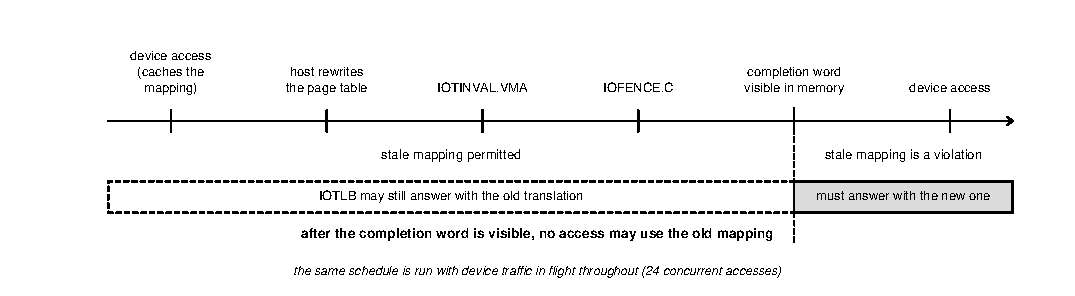
\includegraphics[width=\textwidth]{figures/figB1_ordering.pdf}
\caption{The schedule underlying P5. Before the fence completion is visible the
IOMMU may answer from its cache; after it, it may not.}
\label{fig:order}
\end{figure*}

Each property is decided by observing the physical address the IOMMU emits for a
device transaction, so each is testable without internal visibility.

\textbf{P1 (staleness permitted).} With a page-table entry modified and no
invalidation issued, a transaction may be answered with the old translation.
This is the control: it confirms the cache is active, so the later properties
are not vacuously satisfied by an implementation that never caches.

\textbf{P2 (effectiveness).} After an unscoped invalidation, a transaction to
the affected page is answered with the new translation, and the IOMMU has
re-read the page tables to obtain it.

\textbf{P3 (scope precision).} After an invalidation scoped to one address, a
transaction to that address is answered with the new translation.

\textbf{P4 (scope containment).} The same scoped invalidation does not disturb
other cached translations. P3 and P4 pin the scope from both sides: an
implementation that ignores scope and flushes everything passes P3 and fails P4;
one that ignores the command passes P4 and fails P3.

\textbf{P5 (completion ordering).} Once the fence's completion word is visible,
no subsequent transaction is answered with a translation removed by a command
preceding the fence (Fig.~\ref{fig:order}).

\textbf{P5$'$ (under load).} P5 holds with device transactions in flight across
the whole sequence, not only with the device quiescent.

\section{Method}
We realise the properties against the open RISC-V IOMMU IP published by
Zero-Day Labs~\cite{rviommu}, in a Verilator environment that drives the
device's four AXI interfaces, serves its implicit page-table and command-queue
accesses from a memory image, and observes translated addresses on the
completion port. The environment is described separately~\cite{companion}; what
matters here is that the testbench owns the memory image, so it can rewrite a
page-table entry between two device transactions and can poll for the fence
completion word directly.

Each property becomes a schedule. P1: map a page, access it so the translation
caches, rewrite the leaf entry to a different physical page, access again,
require the old address. P2: as P1 with an unscoped \cmd{IOTINVAL.VMA}
first, requiring the new address \emph{and} evidence of a walk. P3/P4: cache two
pages, rewrite both entries, invalidate only the first, require the first
refreshed and the second unchanged. P5: rewrite an entry, enqueue the
invalidation and then \cmd{IOFENCE.C} with a completion address, poll the
image for the completion word, then issue the transaction.

Three details make the schedules trustworthy. The page-table rewrite is made
directly in the memory image, not through any hardware path, so a cached
translation can only be refreshed by the IOMMU re-reading the entry.
``Refreshed'' is distinguished from ``happened to be right'' by counting the
implicit accesses the IOMMU issues on its data-structure port. And the fence
completion is observed the way software observes it---by polling the image at
the address given in the command---rather than by watching an internal signal,
which may assert before the word appears.

P5$'$ uses two processes. One issues twenty-four transactions to the affected
page with a short gap between them. The other waits, enqueues the invalidation
and fence, and sets a flag when the completion word appears. Transactions
completing after the flag are checked; those before it are unconstrained. The
test records the split, so a run in which too few transactions were post-fence
is visible rather than silently weak.

\section{Results}

\begin{table}[!t]
\caption{Ordering properties on the implementation under test}
\label{tab:props}
\centering\footnotesize
\begin{tabular}{llc}
\toprule
 & Property & Result \\
\midrule
P1  & staleness permitted before invalidation & holds \\
P2  & invalidation is effective (forces re-walk) & holds \\
P3  & scoped invalidation refreshes the named page & holds \\
P4  & scoped invalidation leaves other pages cached & holds \\
P5  & no stale translation after fence completion & holds \\
P5$'$ & P5 under twenty-four concurrent transactions & holds \\
\bottomrule
\end{tabular}
\end{table}

All six hold (Table~\ref{tab:props}); thirteen checks in the wider suite belong
to this family. Under P2 the invalidated access re-reads the page tables, which
the environment confirms by counting implicit accesses. Under P4 the untouched
page is still answered from the cache with its original translation, so the
scope is neither too wide nor ignored. A variant of P2 that caches four
pages---filling the IOTLB in this configuration---and invalidates all of them
refreshes all four. Under P5 the completion word appears twelve cycles after the
command is enqueued. Under P5$'$, twenty of the twenty-four transactions
complete after the completion word is visible and none uses the stale
translation (Fig.~\ref{fig:conc}, upper row).

\begin{figure*}[!t]
\centering
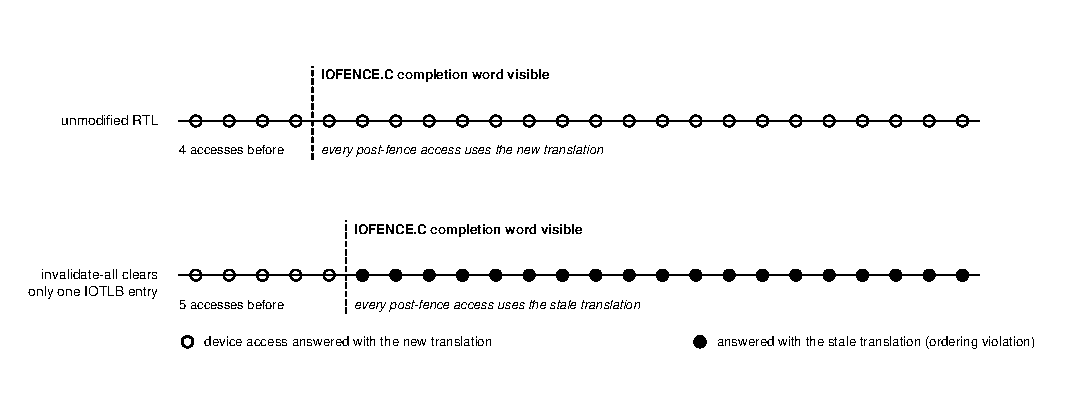
\includegraphics[width=\textwidth]{figures/figB2_concurrent.pdf}
\caption{P5$'$ on the unmodified design and with a partial-flush defect
injected. Each marker is one device transaction; the property constrains only
those right of the dashed line. The defect is invisible before the fence and
total after it.}
\label{fig:conc}
\end{figure*}

\section{Do the Tests Discriminate?}
A suite in which everything passes is worth little unless it fails when it
should. We injected two invalidation defects, each a single scripted edit to the
RTL, and reran.

The first leaves the IOTLB entry uncleared when a matching invalidation arrives.
Six checks fail, P2 among them.

The second makes an unscoped invalidation clear only the first IOTLB entry,
leaving the rest stale---the shape of a real partial-flush bug. Four checks
catch it. A suite that invalidated and rechecked a single page would have passed
it, because the page it checked would be the entry that was cleared; the
multi-page form of P2 is the only thing separating a suite that catches this
from one that does not. Under P5$'$ the same defect produces nineteen stale
translations out of nineteen post-fence transactions (Fig.~\ref{fig:conc}, lower
row): once the surviving entry is the one the device is using, every transaction
after the fence is wrong.

Both defects leave the design fully functional---it translates, walks, and
faults correctly---which is a fair model of how such a bug reaches silicon.
Neither is caught by any test outside this property family.

\section{The Guarantee Is Incidental}
The implementation satisfies P5, but the reason deserves scrutiny. Its command
handler implements \cmd{IOFENCE.C} by writing the completion word when the
command is processed; it does not wait for preceding commands to retire. The
source states the reasoning: because every command the design implements
completes immediately, there is nothing to wait for.

That is sound for the current feature set and unsound as a design property.
\cmd{IOFENCE.C} exists to order commands whose effects are not immediate. The
specification's ATS invalidation commands, absent here, require a round trip to
a device and are exactly that case; so is any future command whose effect is
pipelined. When one is added, P5 stops following from the structure of the
design, and nothing will notice: the fence will keep completing immediately and
the tests will keep passing until a command is slow enough for the window to
open. The fence's predecessor-read and predecessor-write bits are also marked
unimplemented.

This is the practical value we claim. P5 is satisfied today; kept in a
regression suite it becomes a guard on the assumption that makes it true.

\section{Applying the Properties Elsewhere}
Nothing in P1--P5$'$ is specific to RISC-V. Each needs three capabilities any
IOMMU offers: a way to cache a translation, a way to invalidate it, and a way to
learn the invalidation took effect. An ARM SMMU offers the latter two as
\texttt{TLBI} commands and a synchronisation command polled in a consumer
register; an Intel VT-d unit offers invalidation descriptors and an
invalidation-wait descriptor that writes a status word to memory, close enough
to \cmd{IOFENCE.C} that the P5 schedule transfers almost unchanged. The
scoping behind P3 and P4 maps onto those architectures' domain- and
address-selective invalidations. What must be rebuilt per target is the
observation path, and that is work any team verifying the design has already
done; added to an existing environment the family is a few hundred lines.

Two assumptions need revisiting on a deeper pipeline. P5$'$ infers that a
transaction observed after the fence word appeared was decided after it, which
needs an extra argument on a design that speculates on translations or reorders
completions. And a design with multiple independent translation caches needs P4
restated over each, since an invalidation reaching one and not another is
precisely the defect it targets.

\section{Limitations}
One implementation, and a negative result in that no violation was found. The
properties are operational, not formal, and we do not claim completeness. Only
first-stage invalidation is exercised: \cmd{IOTINVAL.GVMA}, \cmd{IODIR},
identifier-scoped invalidation and ATS invalidation are not. Concurrency uses a
single device stream; multiple devices with distinct identifiers would be
stronger. One simulator, one cache configuration---the four-page form of P2 is
sized to this IOTLB. Fault injection measures whether the tests catch the
defects we thought to inject, which is evidence of discrimination but not a
bound on what they would miss.

\section{Reproducibility}
The tests, the environment, and the fault-injection harness are released under a
permissive licence and run with open tools; a single command builds the design,
runs the suite, and reproduces the injected-defect results.

\section{Conclusion}
The ordering obligation an IOMMU owes to an operating system's unmap path is
testable cheaply against RTL, and it is not covered by CPU-side work on
translation-aware ordering. Five properties, expressed as schedules over the
command interface and decided at the completion port, pin the boundary from both
sides. An open RISC-V IOMMU satisfies all of them, including under concurrent
traffic, and two injected invalidation defects are caught. Its fence, however,
does not wait for preceding commands: compliance rests on every implemented
command being immediate, a fact about today's feature set rather than a
guarantee of the design.

\begin{thebibliography}{9}
\bibitem{thunderclap} A.~T.~Markettos \emph{et al.}, ``Thunderclap: Exploring
vulnerabilities in operating system IOMMU protection via DMA from untrustworthy
peripherals,'' in \emph{NDSS}, 2019.
\bibitem{coatcheck} D.~Lustig, G.~Sethi, M.~Martonosi, and A.~Bhattacharjee,
``COATCheck: Verifying memory ordering at the hardware--OS interface,'' in
\emph{ASPLOS}, 2016.
\bibitem{transform} N.~Manerkar, D.~Lustig, M.~Martonosi, and A.~Bhattacharjee,
``TransForm: Formally specifying transistency models and synthesizing enhanced
litmus tests,'' in \emph{ISCA}, 2018.
\bibitem{rtlcheck} Y.~A.~Manerkar, D.~Lustig, M.~Martonosi, and M.~Pellauer,
``RTLCheck: Verifying the memory consistency of RTL designs,'' in \emph{MICRO},
2017.
\bibitem{realitycheck} Y.~A.~Manerkar, D.~Lustig, and M.~Martonosi,
``RealityCheck: Bringing modularity, hierarchy and abstraction to automated
microarchitectural memory consistency verification,'' arXiv:2003.04892, 2020.
\bibitem{qed} ``QED: Scalable verification of hardware memory consistency,''
arXiv:2404.03113, 2024.
\bibitem{iotlb} N.~Amit, M.~Ben-Yehuda, and B.-A.~Yassour, ``IOMMU: Strategies
for mitigating the IOTLB bottleneck,'' in \emph{WIOSCA}, 2010.
\bibitem{rviommu} Zero-Day Labs, ``RISC-V IOMMU IP,'' commit \texttt{18ad30a}.
[Online]. Available: \url{https://github.com/zero-day-labs/riscv-iommu}
\bibitem{companion} M.~Timbadiya, ``Verifying the RISC-V IOMMU: an open
verification environment and a fault-injection evaluation,'' companion paper.
\end{thebibliography}

\end{document}
